\documentclass[border=10pt, tikz]{standalone}
\usetikzlibrary{arrows.meta}

\definecolor{curveblue}{HTML}{B2D7EA} 
\definecolor{jumpred}{HTML}{E97AB1}   
\definecolor{textdark}{HTML}{222222}

\begin{document}
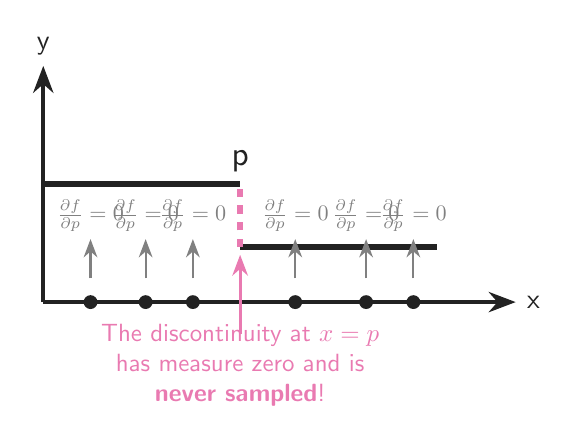
\begin{tikzpicture}[font=\sffamily, >=Stealth]

    % Axes
    \draw[line width=1.5pt, ->, textdark] (0,0) -- (6,0) node[right] {x};
    \draw[line width=1.5pt, ->, textdark] (0,0) -- (0,3) node[above] {y};

    % Step Function
    \draw[line width=2pt, textdark] (0,1.5) -- (2.5,1.5);
    \draw[line width=2pt, textdark] (2.5, 0.7) -- (5, 0.7);
    \draw[jumpred, line width=2pt, dashed] (2.5, 0.7) -- (2.5, 1.5);
    \node[above, textdark, scale=1.2] at (2.5, 1.5) {p};
    
    % MC Samples (The "Misses")
    \foreach \x in {0.6, 1.3, 1.9, 3.2, 4.1, 4.7} {
        \fill[textdark] (\x, 0) circle (2.5pt);
        \draw[->, gray, line width=0.8pt] (\x, 0.3) -- (\x, 0.8);
        \node[above, scale=0.8, text=gray] at (\x, 0.8) {$\frac{\partial f}{\partial p}=0$};
    }

    % The "Missing" Information
    \node[jumpred, scale=0.9, align=center] at (2.5, -0.8) {The discontinuity at $x=p$ \\ has measure zero and is \\ \textbf{never sampled}!};
    \draw[jumpred, ->, line width=1pt] (2.5, -0.4) -- (2.5, 0.6);

\end{tikzpicture}
\end{document}
